\section{Architektur}
\subsection{System Übersicht}
Für die Umsetzung der Anwendung gibt es zwei Optionen. Man kann zwischen einer Native App, also einer klassische Client-Server Anwendung, oder eine Web Anwendung, entscheiden. \\

Native Apps haben zwar einige Vorteile. Die Integration mit anderen Anwendungen ist so zum Beispiel einfacher. Zudem wäre die Monetarisierung auch um einiges einfacher, denn eine Native App kann sehr gut im App Store platziert werden. So steigt auch gleich die Bekanntheit der Applikation\footcite{native_app}. \\

Die Entscheidung bei der Entwicklung von Aufgaben-Coach fiel jedoch sehr schnell auf eine Web Anwendung. Viele Schulen haben zwar Apple iPads im Einsatz. Trotzdem kann es Schulen geben, welche mit Android Tablets arbeiten. Mit einer Native App müsste für jedes Betriebssystem ein separates Programm erstellt werden.\\

Hinzu kommt noch die Anforderung der Lehrer. Da diese hauptsächlich auf Notebooks oder Desktop PCs arbeiten, müsste für sie auch eine separate Anwendung entwickelt werden. Mit einer Web Anwendung hat man den Vorteil, nur eine Anwendung entwickeln zu müssen, auf welche alle Benutzer Zugriff haben.\\

Ein weiterer Vorteil von Web Anwendungen ist, dass im vorhinein kein Programm auf dem Device installiert werden muss. Alles, was ein Benutzer braucht, ist ein Internetzugang und ein Tablet. Dies senkt zugleich die Supportkosten der Schule, da so keine Zeit für die Installation oder das Updaten verbraucht wird.

\begin{figure}[H]
\begin{center}
	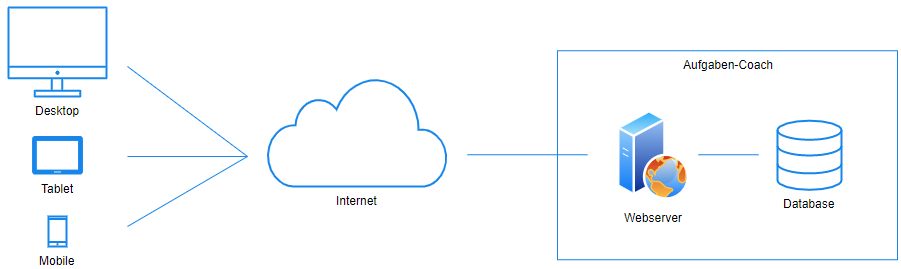
\includegraphics[width=\textwidth, keepaspectratio]{images/system_overview.png}
	\caption{System Overview}
	\label{fig:system_overview}
\end{center}
\end{figure}


\subsection{Domain Model}
In der Abbildung \ref{fig:domain_model_full} ist das vollständige Domain Model abgebildet. Dem Leser soll so ein Überblick über die einzelnen Teilgebiete der Anwendung gegeben werden.

\begin{landscape}

\begin{minipage}{\textwidth}
	\begin{figure}[H]
		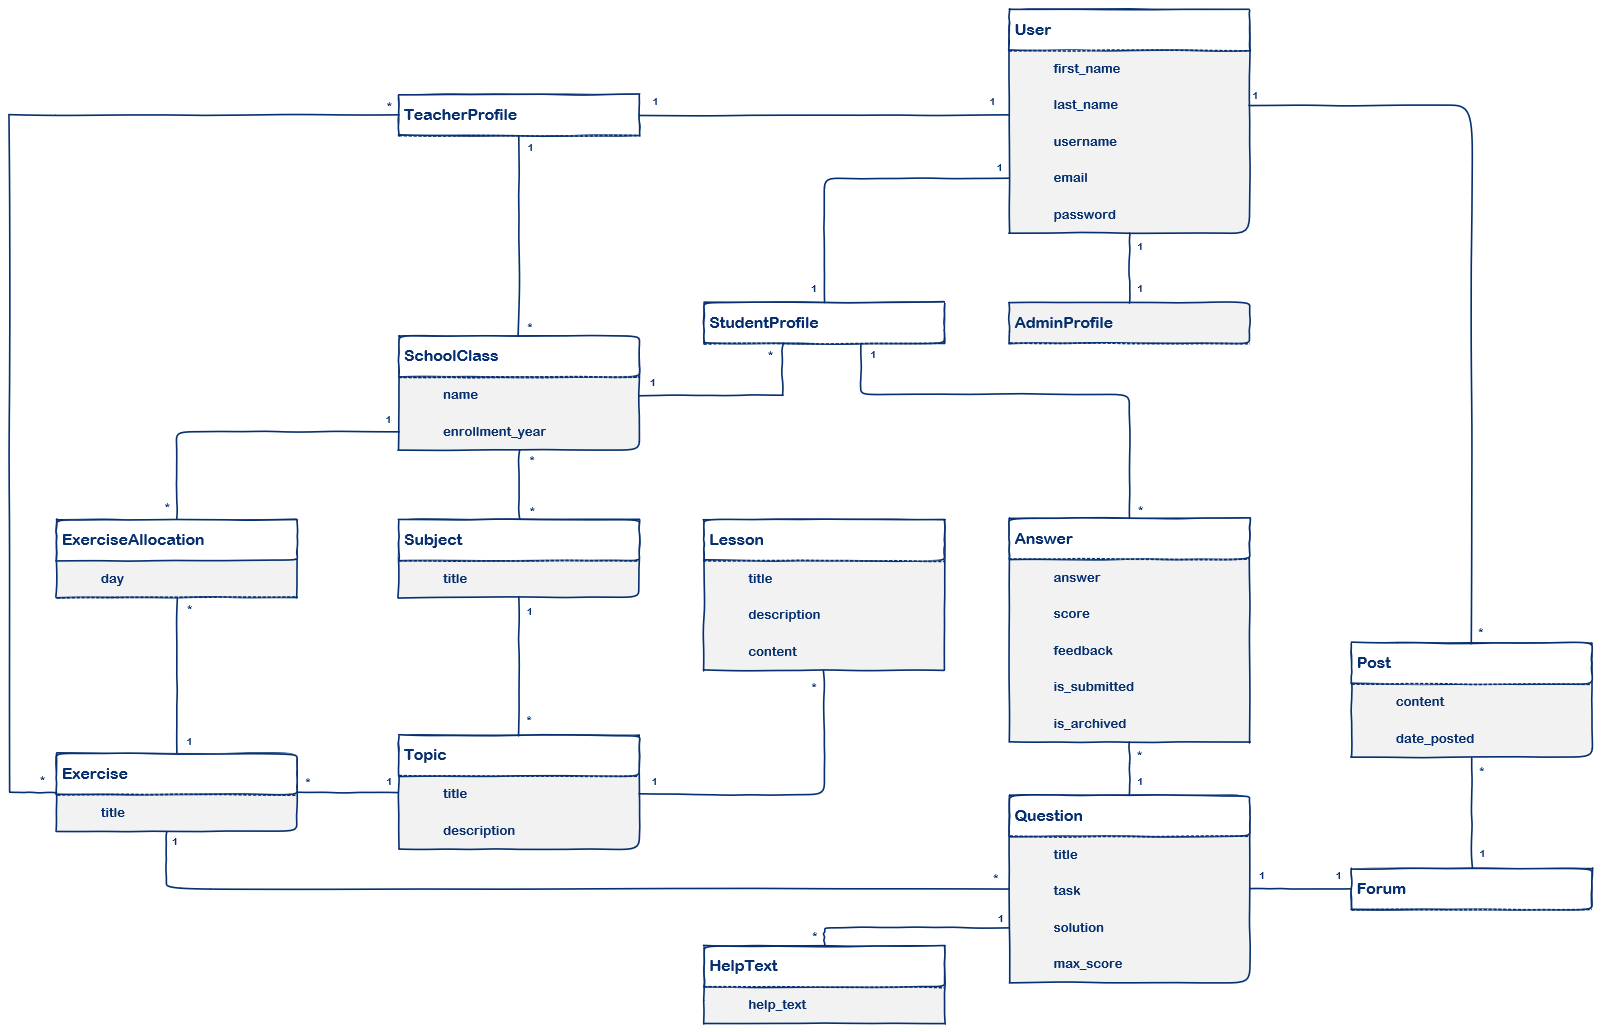
\includegraphics[width=1.4\textwidth, keepaspectratio]{images/domain_model_full.png}
  		\caption{Vollständiges Domain Model}
		\label{fig:domain_model_full}
	\end{figure}
\end{minipage}

\end{landscape}

%TODO SchoolClass im Domain Model zeigen
\subsubsection*{School}
Ein zentraler Punkt der Anwendung ist die Schule und das User Management. Die User sind einer der drei Rollen Student, Teacher oder Admin zugeteilt. Da jede Rolle unterschiedliche Rechte hat, konnte nicht das Standard User Model von Django selbst verwendet werden. \\
Es stehen drei Möglichkeiten zur Verfügung, wie unterschiedliche User Rollen implementiert werden können.

\begin{enumerate}
	\item Unterscheidung der User anhand eines Boolean Flags
	\item Unterscheidung der User anhand eines Choices Field 
	\item Erstellung eines Profile Models mit einer 1 zu 1 Beziehung zum User Model
\end{enumerate}

Die erste Variante hat den Vorteil, dass ein User mehrere Rollen gleichzeitig haben kann. Im Gegensatz zur ersten Variante kann ein User bei der zweiten Variante nur eine Rolle annehmen. Diese beiden Varianten haben jedoch den Nachteil, dass jeder User die gleichen Daten hat. Möchte man einem Schüler eine Matrikelnummer zuweisen, existiert dieses Feld implizit auch für alle Lehrer und Admins. \\
Um diesem Problem aus dem Weg zu gehen, entschied man sich für die dritte Variante. Pro Rolle existiert ein Profile Model. Möchte man nur einer bestimmten Rolle ein Feld zuweisen, so kann dieses Feld im entsprechenden Profile Model hinzugefügt werden\footcite{django:user_types}. \\

\begin{figure}[H]
	\begin{center}
	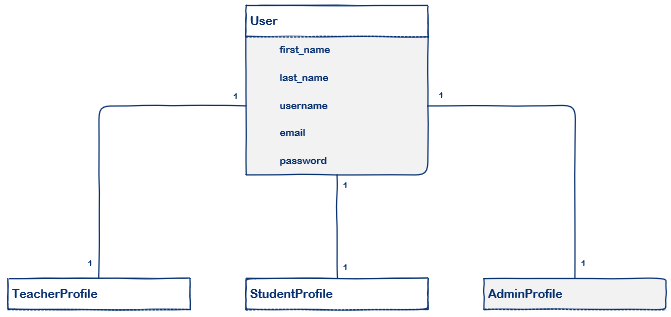
\includegraphics[width=\textwidth, keepaspectratio]{images/domain_model_user.png}
	\caption{Domain Model - User Abschnitt}
	\label{fig:domain_model_user}
	\end{center}
\end{figure}

Der Admin kann als einziger User Typ für sich alleine existieren. Schüler und Lehrer werden Klassen zugewiesen. Ein Lehrer kann gleichzeitig mehreren Klassen zugewiesen sein, ein Schüler kann sich jedoch nur in einer Klasse befinden. Für den aktuellen Stand reicht diese Funktionalität aus. Es gibt jedoch den Use Case, in welchem Schüler aus unterschiedlichen Klassen Fächer zusammen belegen. Dies ist zum Beispiel der Fall, wenn Migrationskinder aus unterschiedlichen Klassen zusammen kommen und gemeinsam ein Deutsch Nachhilfe Fach besuchen. Für diesen Fall kann man dem Student Profile ein Boolean Flag zuweisen. Falls dieses Flag gesetzt ist, hat der Schüler Zugriff auf Nachhilfe Fächer. \\

Wenn dieses Projekt als Startup weiter verfolgt wird, dann würde pro Schule eine neue Instanz der Anwendung deployed werden. So entstehen keine Multi Tenancy Probleme. Möchte man in Zukunft jedoch einen Multi Tenancy Ansatz verfolgen, müsste das Domain Model dementsprechend angepasst werden. Ein möglicher Lösungsansatz wäre, wenn jeder Schule eine eigene Subdomain, wie zum Beispiel schule-gossau.aufgaben-coach.ch, vergeben würde. Anhand der Subdomain können dann die einzelnen User identifiziert werden\footcite{django:multi_tenancy}.

\newpage
%TODO User, StudentProfile und TeacherProfile entfernen
\subsubsection*{Study Content}
Ein zentraler Punkt dieser Anwendung sind die Schulfächer. Pro Subject gibt es mehrere Topics. Topics wiederum können mehrere Lessons haben. \\ 

\begin{figure}[H]
\begin{center}
	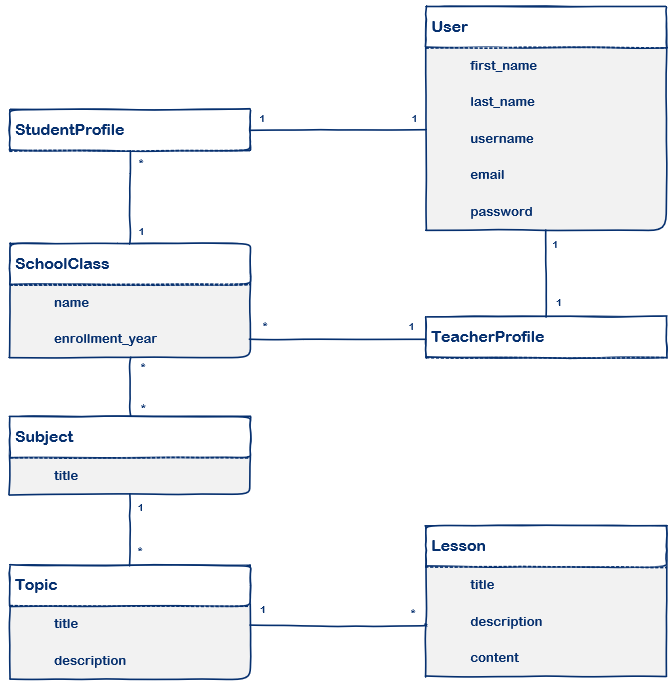
\includegraphics[width=\textwidth, keepaspectratio]{images/domain_model_study_content.png}
	\caption{Domain Model - Schulfächer}
	\label{fig:domain_model_study_content}
\end{center}
\end{figure}


Ein Subject kann einer Klasse zugewiesen werden. Erst dann hat die Klasse Zugriff auf Topics und Lessons. Im Moment ist es nicht möglich, einzelne Topics oder Lessons freizuschalten. Möchte man diese Funktionalität in Zukunft jedoch haben, muss eine neue Zwischentabelle in der Datenbank erstellt werden.

\newpage
\subsubsection*{Exercise}
Das Herzstück der Anwendung sind die Exercises. Lehrer können Übungen erstellen, welche aus mehreren Teilaufgaben bestehen, welche wiederm mehrere Hilfestellungen haben. 

\begin{figure}[H]
\begin{center}
	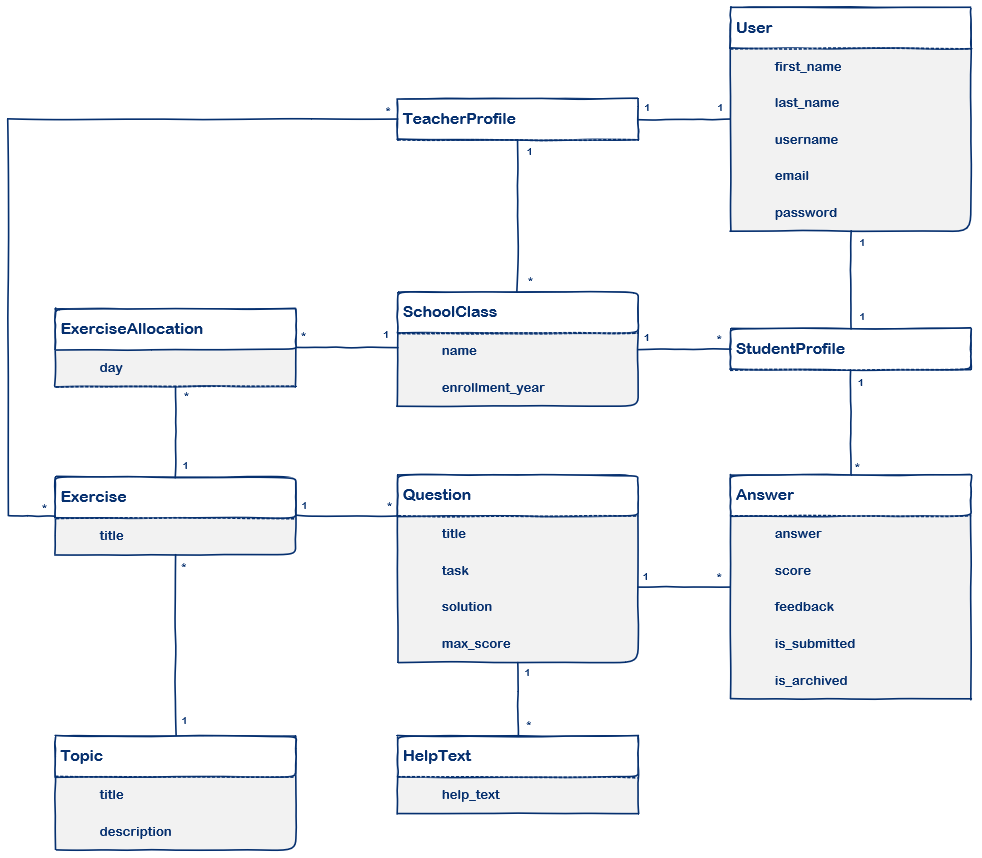
\includegraphics[width=\textwidth, keepaspectratio]{images/domain_model_exercise.png}
	\caption{Domain Model - Aufgaben}
	\label{fig:domain_model_exercise}
\end{center}
\end{figure}

Die Tabelle Answer dient zur Speicherung der Antworten von Schülern. Die beiden Felder ''is\_submitted'' und ''is\_archived'' sind für den Status der Aufgaben. Ist eine Aufgabe submitted, also abgegeben, kann sie nicht weiter vom Schüler bearbeitet werden. Erst wenn Aufgaben abgegeben sind, können sie vom Lehrer angeschaut werden. \\ 
Wurden die Aufgaben vom Lehrer korrigiert, bekommen sie den Status ''is\_archived''.

\newpage
\subsubsection*{Forum}
Für jede Frage in einer Übung gibt es ein Forum. Die Schüler haben einen Ort, in welchem Fragen gestellt werden können. Da es für jede Frage ein Forum gibt, werden die Schüler auch nicht von anderen Forumsbeiträgen abgelenkt.
\begin{figure}[H]
\begin{center}
	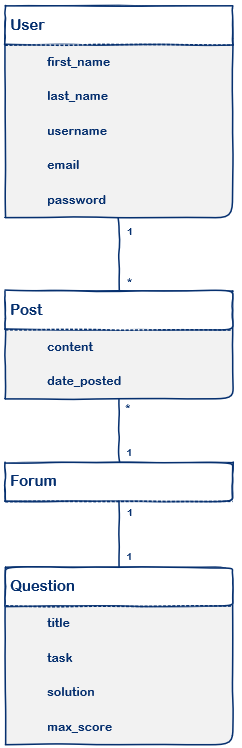
\includegraphics[width=0.3\textwidth, keepaspectratio]{images/domain_model_forum.png}
	\caption{Domain Model - Forum}
	\label{fig:domain_model_forum}
\end{center}
\end{figure}


\subsection{Tools und Frameworks}
Bei der Wahl von Technologien, Tools und Frameworks achtete man besonders darauf, dass die entsprechenden Tools auch in der Zukunft noch supported werden. Dazu wurde geschaut, ob und wie gross die Community hinter einzelnen Tools ist und wie gut die Tools dokumentiert sind.

\subsubsection*{Programmiersprache}
Für das Web Development gibt es mehrere Programmiersprachen, die zur Auswahl stehen. Die Wohl bekanntesten darunter sind:

%https://en.wikipedia.org/wiki/Web_framework

\begin{itemize}
	\item Python (Django / Flask)
	\item C\# (ASP.NET Core)
	\item Java (Spring)
	\item JavaScript (Express.js / Node.js / Sails.js)
	\item PHP (CakePHP / CodeIgniter / Laravel)
	\item Perl (Catalyst / Mojolicious)
	\item Ruby (Ruby on Rails)
\end{itemize}

%TODO Satzstellung anschauen

Gemäss Developer Survey Results\footcite{developer_survey_results} von Stack Overflow ist Python (41.7\%) etwas beliebter als Java (41.1\%). Nur JavaScript (67.8\%) ist noch bekannter. In den letzten Jahren ist die Bekanntheit von Python noch weiter gestiegen. \\

Die Wahl der Programmiersprache fiel schnell auf Python, da bereits etwas KnowHow vorhanden ist. Man geht aber davon aus, dass Python in Zukunft noch an Beliebtheit steigt und man weiterhin damit arbeiten kann.


\subsubsection*{Web Framework}
Mit Python hat man die Auswahl von verschiedenen Web Frameworks. Gemäss einer Umfrage von JetBrains\footcite{python_survey_results} wird die Frage ''What web frameworks / libraries do you use in addition to Python?'' mit dem Kommentar ''Django and Flask continue to be by far the most popular Python web frameworks.'' zusammengefasst. \\
Laut dieser Umfrage verwenden 43\% der Entwickler  Django als Web Framework. Flask folgt dicht darauf mit 41\%. Das nächst bekannteste Framework ist Tornado mit nur noch 6\%. \\
Bei der Evaluation konzentrierte man sich deshalb hauptsächlich auf Django und Flask. Mit bekannteren Frameworks hat man den Vorteil, dass es einfacher ist, Hilfe und gute Dokumentationen zu finden. Mit weit verbreiteten Technologien kann man auch davon ausgehen, dass diese noch längere Zeit bestehen bleiben.  \\ 

%TODO zitat einbauen
Flask\footcite{flask:foreword} beschreibt sich selber mit den Worten:

\begin{displayquote}
Flask is a lightweight WSGI web application framework. It is designed to make getting started quick and easy, with the ability to scale up to complex applications. It began as a simple wrapper around Werkzeug and Jinja and has become one of the most popular Python web application frameworks. \\
Flask offers suggestions, but doesn't enforce any dependencies or project layout. It is up to the developer to choose the tools and libraries they want to use. There are many extensions provided by the community that make adding new functionality easy.
\end{displayquote}

Bei der Studienarbeit verwendete man bereits Flask zum Erstellen einer Web Anwendung. Flask ist sicherlich ein gutes Framework, sonst würde es nicht von 41\% der Entwickler genutzt. Der grosse Vorteil dieses Frameworks ist, dass man als Entwickler relativ frei ist, wie man etwas umsetzen möchte. So kommt Flask standardmässig ohne Database Abstraction Layer, Form Validation oder anderen Tools, da bereits Libraries existieren, welche dies erledigen\footcite{flask:design}. Gerade am Anfang kann dies jedoch eher Verwirrung stiften, weil für das selbe Problem mehrere Lösungsmöglichkeiten bereit stehen. \\

Django verfolgt dagegen eher den Ansatz, bereits unterschiedliche Funktionalitäten mitzuliefern, was den Entwicklern Arbeit abnehmen soll. So ist zum Beispiel bereits ein OR-Mapper oder ein Admin Interface integriert\footcite{django:overview}. 
Django hat aber auch ein paar Nachteile. Da einige Entscheidungen bereits vom Framework selber getroffen wurden, ist man als Entwickler nicht mehr ganz so flexibel. Zudem ist Django sehr monolithisch. Bei bestimmten Aufgaben ist vorgegeben, wie diese in Django umgesetzt werden müssen. Hält man sich nicht an den ''Django Way'', kann unter Umständen die gesamte Anwendung nicht deployed werden\footcite{django:advantages_disadvantages}.

In der Studienarbeit konnte man zwar bereits Erfahrung mit Flask sammeln, dennoch entschied man sich für Django. Der Hauptgrund dafür ist, dass das Django Framework als ''Fully Loaded Framework'' daher kommt un so zum Beispiel ein integriertes Admin Interface besitzt.


\subsubsection*{Datenbank}
Aufgrund der ohnehin schon verkürzten Projektlaufzeit entschied man sich, auf die Evaluation eines Datenbanksystems zu verzichten. Während den Modulen Datenbanksysteme 1 \& 2 konnte bereits sehr viel Erfahrungen mit Postgres gesammelt werden. Laut Deployment Statistics\footcite{deploymentstatistics} von Django Sites verwenden 47.7\% aller deployten Sites MySQL als Datenbank. Postgres folgt mit 40.7\%. Das nächst grössere Datenbanksystem ist sqlite mit nur noch 7.6\%.
MySQL wird zwar etwas öfters verwendet. Aus Erfahrung weiss man aber, dass die Funktionen von Postgres die Bedürfnisse dieser Anwendung voll und ganz abdecken, weshalb man Postgres als Datenbanksystem festlegte. \\

Sollte man in Zukunft jedoch ein anderes Datenbanksystem bevorzugen, kann die Migration mit dem Django Management Tool durchgeführt werden \footcite{dbmigration}. 

\subsubsection*{Python Libraries}
Libraries beschreiben


\subsection{Deployment}
Zusätzlich zur System Overview in Abbildung \ref{fig:system_overview}, wird hier das Deployment Diagramm gezeigt. Dieses soll die einzelnen Komponenten aufzeigen.

\begin{figure}[H]
\begin{center}
	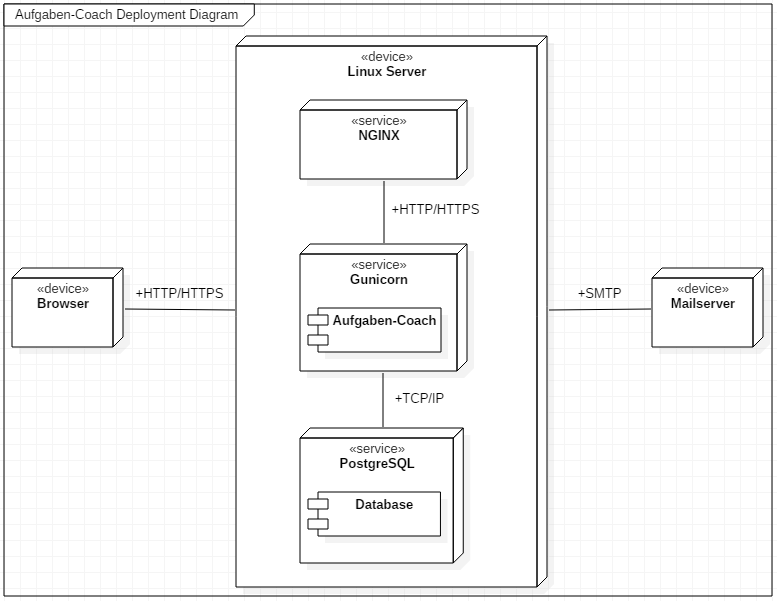
\includegraphics[width=\textwidth, keepaspectratio]{images/deployment_diagram.png}
	\caption{Deployment Diagramm}
	\label{fig:deployment_diagram}
\end{center}
\end{figure}

\subsubsection*{Web Server}
Bei der Evaluation eines Web Servers beschränkte man sich auf NGINX und Apache. Wie man auf einer Statistik von w3techs\footcite{webserver_usage} entnehmen kann, wird in 42\% der Web Server Apache eingesetzt. NGINX kommt mit 31.3\% etwas weniger zum Einsatz. \\

Apache kommt öfters zum Einsatz und ist flexibler als NGINX\footcite{webserver_comparison}. Dennoch entschied man sich für NGINX. Bei dieser Entscheidung achtete man hauptsächlich auf die Performance der beiden Web Server, bei welcher NGINX in den Kategorien ''Requests per second'', ''Time per request'' und ''Transfer rate'' durchschnittlich besser abschnitt\footcite{webserver_performance}.

\subsection*{Web Server Gateway Interface}
Während der Entwicklungsphase wurde der Development Server, welcher direkt mit dem Django Framework mitgeliefert wird, verwendet. In der produktiven Umgebung reicht dies jedoch nicht mehr aus, weshalb ein \gls{wsgi} eingesetzt wird. Dieser beschreibt, wie der Web Server mit einer Web Anwendung kommuniziert. Anfragen an den Web Server werden zur Web Anwendung geleitet. Sobald der Request bearbeitet wurde, wird die Response an den Web Server zurück geschickt\footcite{wsgi_description}.

